\subsubsubsubsection{Config reader}
\begin{figure}[h]
\centering
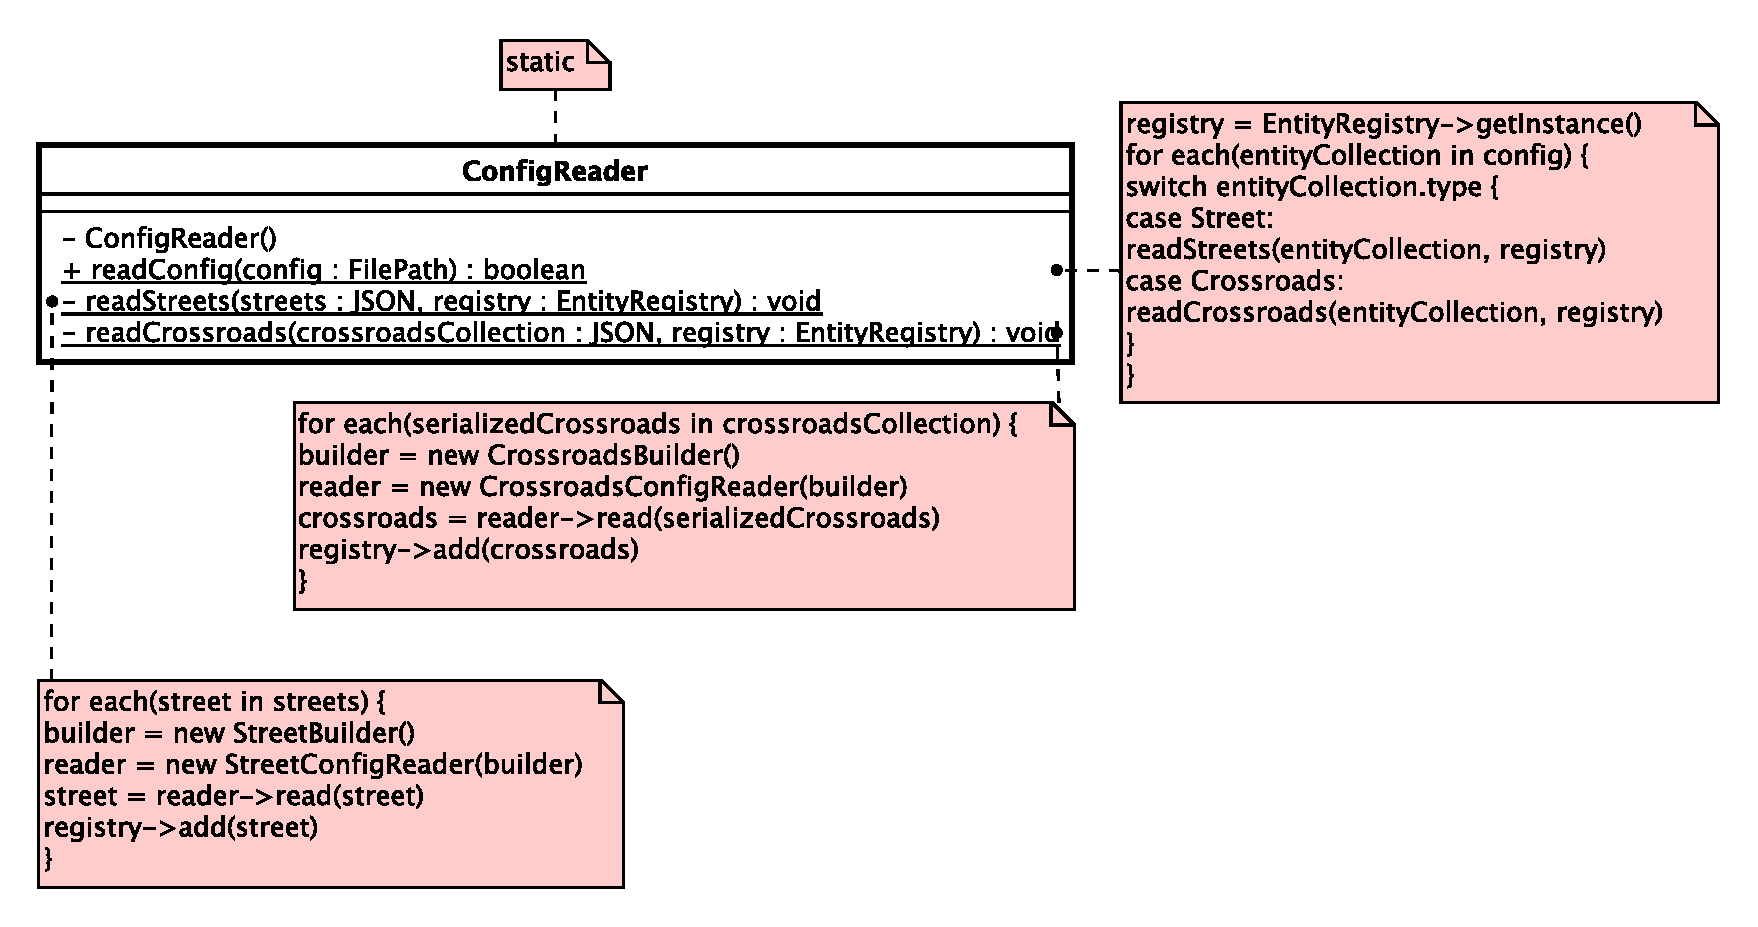
\includegraphics[scale=0.6,keepaspectratio]{images/solution/app/backend/config_reader.eps}
\caption{\pReactive::ConfigReader}
\label{fig:sd-app-district-starter}
\end{figure}
\FloatBarrier
\begin{itemize}
  \item \textbf{\descr} \\
  It has the responsibility to parse a configuration file.
  It is a static class because it is composed of only static methods.
  \item \textbf{\ops}
  \begin{itemize}
    \item \texttt{ConfigReader()} \\
    Private and unique constructor because the class provides only static methods 
    so there are no reasons a client creates instances of it.
    \item \texttt{\underline{readConfig(config: FilePath) : boolean}} \\
    Parses a configuration file.
    Returns true if the process completes neatly, false otherwise.
    \item \texttt{\underline{readStreets(streets : JSON, registry : EntityRegistry) : boolean}} \\
    Parses a serialization of streets and appends them the the district.
    Returns true if the process completes neatly, false otherwise.
    \item \texttt{\underline{readCrossroads(crossroadsCollection : JSON, registry : EntityRegistry) : boolean}} \\
    Parses a serialization of crossroads and appends them the the district.
    Attaches each crossroads to the relative traffic light
    if specified so in the configuration file. 
    Returns true if the process completes neatly, false otherwise.
  \end{itemize}
\end{itemize}
